\documentclass[border=2pt]{standalone}
\usepackage[dvipsnames,svgnames,x11names]{xcolor}
\usepackage{tikz}
\usetikzlibrary{arrows.meta}
\begin{document}
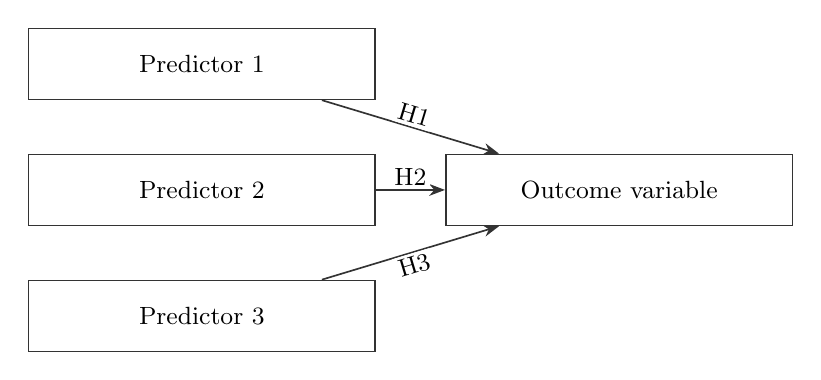
\begin{tikzpicture}[font=\small,>=Stealth,x=53.0mm,y=16.0mm]
\node[rectangle,fill=white,draw=black!80,text=black,line width=0.6pt,minimum height=9mm,inner xsep=7pt,inner ysep=4.5pt,align=center,text width=39.1mm,execute at begin node={\hyphenpenalty=10000\relax}] (x1) at (0,0) {Predictor 1};
\node[rectangle,fill=white,draw=black!80,text=black,line width=0.6pt,minimum height=9mm,inner xsep=7pt,inner ysep=4.5pt,align=center,text width=39.1mm,execute at begin node={\hyphenpenalty=10000\relax}] (x2) at (0,-1) {Predictor 2};
\node[rectangle,fill=white,draw=black!80,text=black,line width=0.6pt,minimum height=9mm,inner xsep=7pt,inner ysep=4.5pt,align=center,text width=39.1mm,execute at begin node={\hyphenpenalty=10000\relax}] (x3) at (0,-2) {Predictor 3};
\node[rectangle,fill=white,draw=black!80,text=black,line width=0.6pt,minimum height=9mm,inner xsep=7pt,inner ysep=4.5pt,align=center,text width=39.1mm,execute at begin node={\hyphenpenalty=10000\relax}] (y) at (1,-1) {Outcome variable};
\draw[->,draw=black!80,line width=0.6pt] (x1) -- node[pos=0.5,above,sloped,fill=white,inner sep=1.2pt] {H1} (y);
\draw[->,draw=black!80,line width=0.6pt] (x2) -- node[pos=0.5,above,fill=white,inner sep=1.2pt] {H2} (y);
\draw[->,draw=black!80,line width=0.6pt] (x3) -- node[pos=0.5,below,sloped,fill=white,inner sep=1.2pt] {H3} (y);
\end{tikzpicture}
\end{document}
